\documentclass{beamer}
\usepackage[utf8]{inputenc}
\usepackage{graphicx}
\usepackage{url}

\author[Sowmya Vajjala]{Instructor: Sowmya Vajjala}


\title[LING 120]{LING 120: \\ Language and Computers}
\subtitle{Semester: Fall '17}

\date{8 November 2017}

\institute{Iowa State University, USA}

%%%%%%%%%%%%%%%%%%%%%%%%%%%

\begin{document}

\begin{frame}\titlepage
\end{frame}

\begin{frame}
\frametitle{Outline}
\begin{itemize}
\item Recap of last class
\item Speech Synthesis
\item Group exercise on scoring speech for proficiency
\item Next class: Conclusion of speech processing
\end{itemize}
\end{frame}

\begin{frame}
\begin{center}
\Large Automatic Speech Recognition - Recap
\end{center}
\end{frame}

\begin{frame}
\frametitle{ASR general process}
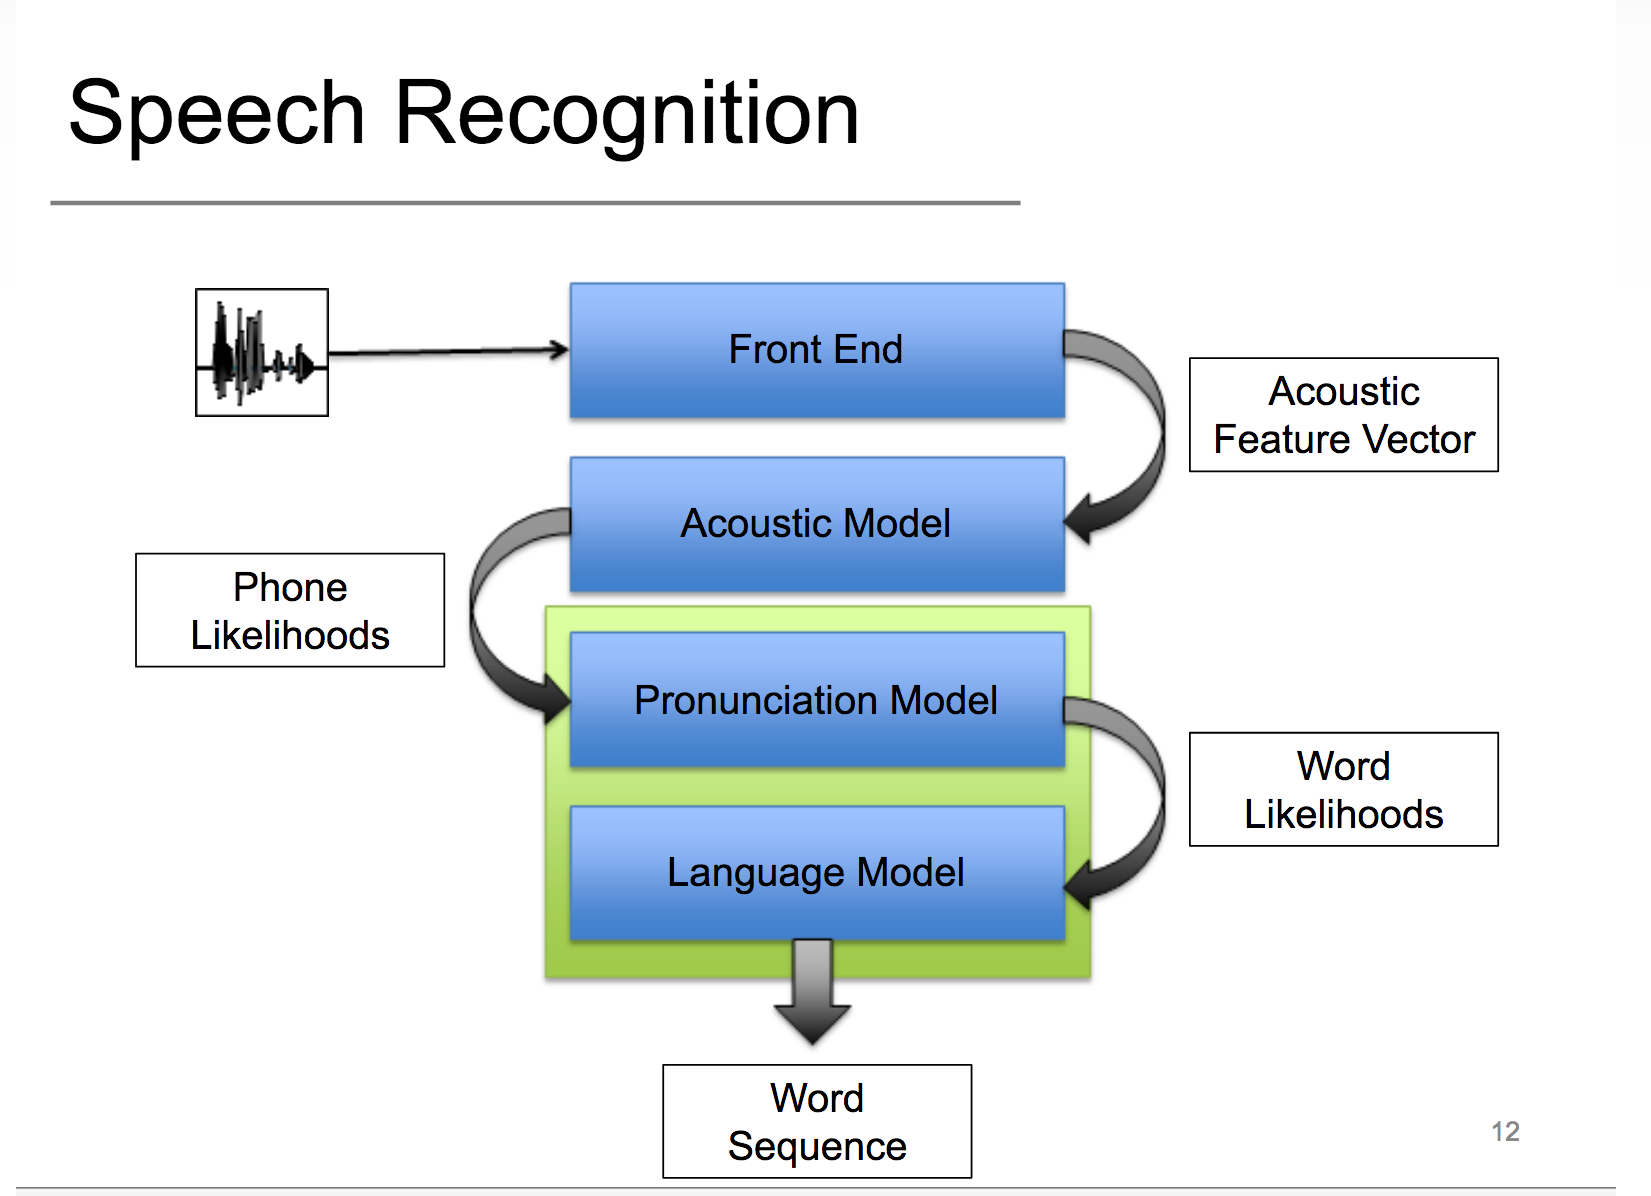
\includegraphics[width=0.9\textwidth]{asr.png}
\\ \tiny source: Andrew Rosenburg's Speech processing lecture.
\end{frame}

\begin{frame}
\frametitle{Evaluation of ASR}
\begin{itemize}
\item Word Error Rate
\item Sentence Error Rate
\item In the case of dialog systems involving spoken input: concept error rate
\end{itemize}
\end{frame}

\begin{frame}
\frametitle{Question from last class}
\begin{itemize}
\item Q: Code-switching refers to people switching between languages while speaking or writing. It is not very common in US, but in multi-lingual societies, it is quite common. What or how do you think ASR systems should be tuned to such scenarios? 
\pause \item A: the answer I was expecting to see: Record code-mixed conversations and use that for acoustic-pronunciation-language models instead of using one language!
\pause \item Microsoft Research-India's CodeMixing project: \url{https://pocomixmaadi.wordpress.com/} and the post on Pronunciation modeling for Code-mixing - \url{https://goo.gl/ijiK9M}
\end{itemize}
\end{frame}

\begin{frame}
\frametitle{ASR news from Yesterday}
Identifying the songs that are playing in the background!
\begin{itemize}
\item http://mashable.com/2017/11/07/google-assistant-android-roll-out
\end{itemize}
\end{frame}

\begin{frame}
\begin{center}
\Large Speech Synthesis
\\ \tiny source: Speech Synthesis, Chapter 8 in Speech and Language Processing by Jurafsky and Martin, 2nd Edition.
\end{center}
\end{frame}

\begin{frame}
\frametitle{What is Speech Synthesis?}
\begin{itemize}
\item What is SS? \pause
\item What is the difference between ASR and SS?\pause
\item Where is it useful? \pause
\item Is it easier than ASR?  \pause
\item What is particularly challenging about SS? \pause
\item What kind of resources and solutions do we need for SS? \pause
\item How would we evaluate SS? 
\end{itemize}
\end{frame}

\begin{frame}
\frametitle{Uses of Speech Synthesis}
\begin{itemize}
\item Dialog agents design
\item Support speech impaired patients with communication aids
\\ \url{https://www.youtube.com/watch?v=UErbwiJH1dI} - Stephen Hawking's speech synthesizer.
\item For people who cannot read (and also perhaps blind people?) - as a means to get information
\item in Language tutoring (to teach how to pronounce correctly?)
\end{itemize}
\end{frame}

\begin{frame}
\frametitle{Challenges for Speech Synthesis}
\begin{itemize}
\item Breaking text down into sounds
\item Mapping sound sequences to correct pronunciation (based on context)
\item Getting the intonation, prosody etc right.
\item Converting to a proper waveform that maps to human language words
\item Not sounding too mechanical
\item Some languages have straight forward pronunciation. Some languages do not. 
\item Some languages Tonal i.e., depending on tone, word meaning changes (e.g. Chinese)
\end{itemize}
\end{frame}

\begin{frame}
\frametitle{Making of a speech synthesizer}
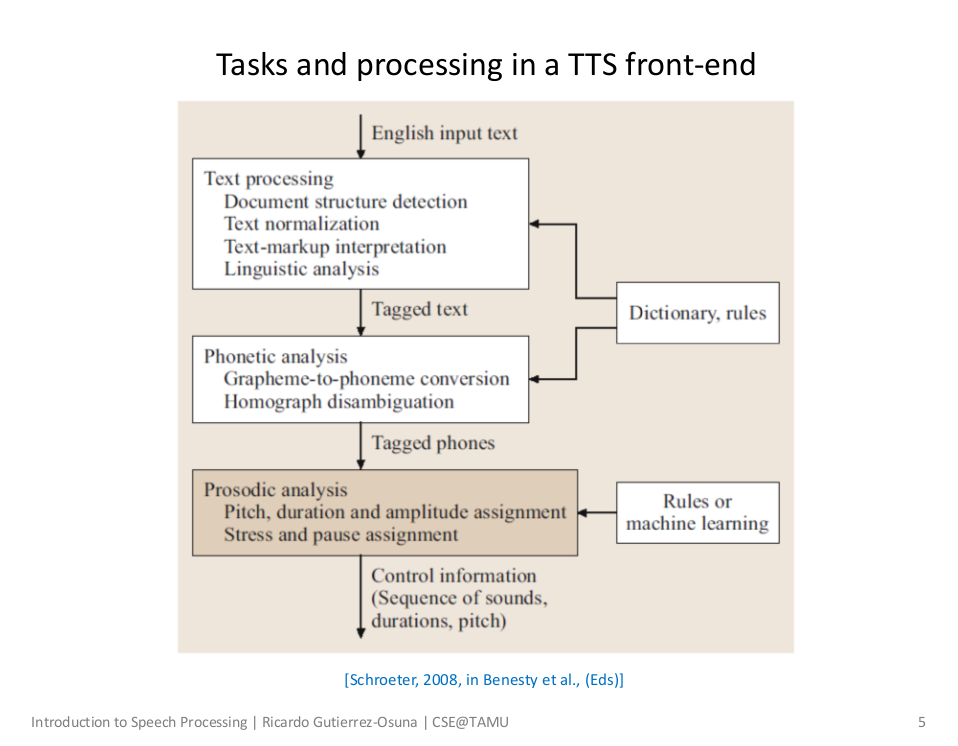
\includegraphics[width=0.9\textwidth]{ss.png}
\end{frame}

\begin{frame}
\frametitle{Some of the important steps}
\begin{itemize}
\item text processing: identifying sentence and word boundaries, pronunciation, abbreviations, symbols (dollar sign) etc. Converting Mr. to Mister, numbers to word form, knowing what to discard (metadata in emails etc) etc. \pause 
\item phonetic analysis: identifying the right pronunciation for the word by analyzing it (converting writing script to phonemes) \pause
\item prosodic analysis: taking care of intonation, emotion and rhythm in speech, identifying phrase boundaries - where to pause etc \pause
\item waveform synthesis based on all the above steps
\end{itemize}
\end{frame}

\begin{frame}
\frametitle{What resources do we need?}
\begin{itemize}
\item text processing: lists of symbols, abbreviations etc, their  word equivalents, sentence and word segmentation programs etc.
\item phonetic analysis: pronunciation dictionaries
\item prosodic analysis: pronunciation dictionaries + knowledge about pronunciation in context.
\item waveform synthesis: usually needs hours and hours of recordings like in ASR (preferably from one person or two, which is not like ASR!), and some way to store the mapping between words/phrases and sounds.
\end{itemize}
\end{frame}

\begin{frame}
\frametitle{There "where do I get so much data" question}
\url{https://research.googleblog.com/2015/09/crowdsourcing-text-to-speech-voice-for.html}
\end{frame}

\begin{frame}
\frametitle{Evaluation of Speech Synthesis}
\begin{itemize}
\item Typically done by human listeners based on aspects such as intelligibility and quality
\item intelligibility: can humans understand the machine utterances correctly?
\item quality: does it sound like a natural human voice? \pause
\item Intelligibility tests: give two similar sounding, confusable rhyming words and check for the differences in machine pronunciation
\item More practical evaluation: make the synthesizer read addresses aloud, give directions etc (whatever is its purpose) and check for intelligibility with this. \pause
\item Quality: ask several people and get a mean opinion score. \pause
\item Comparing 2 systems: play both and ask humans which one is better
\end{itemize}
\end{frame}

\begin{frame}
\frametitle{A historical perspective after this background}
\begin{itemize}
\item Voder, early speech synthesizer from Bell Labs (1939): \url{https://www.youtube.com/watch?v=0rAyrmm7vv0}
\item Ordering a Pizza with a computer voice (1974): \url{https://www.youtube.com/watch?v=94d_h_t2QAA}
\item More such stuff: See the History section in Wikipedia page: \url{https://en.wikipedia.org/wiki/Speech_synthesis}
\end{itemize}
\end{frame}


\begin{frame}
\frametitle{Speech Synthesis in Real World}
\begin{itemize}
\item Google, Microsoft, IBM - all major IT companies have a speech synthesizer software that others can also use in their own programs.
\item Google Translate, Maps have one version of this for multiple languages. (Let us take a look at translate's SS)
\item Siri's responses to you won't happen without some form of synthesis
\item This is not exactly synthesis - but Waze allows you to record your own voice and uses that to give directions later.
\item Synthesizing your own voice back to you?: \url{lyrebird.ai}, \url{goldenspeaker.las.iastate.edu}
\end{itemize}
\end{frame}

\begin{frame}
\frametitle{Attendance Exercise}
Work in groups of 2--4 people
\begin{itemize}
\item We briefly talked about an automated scoring system in text classification class (i.e., classifying English writing into beginners, intermediate, advanced learners) like in exams like GRE, TOEFL etc. 
\item Scenario: Test taker gets a question, they respond with, say, a 1 minute speech on that, and you get the speech file. 
\item If we were to do the same kind of classification system with with these files, what do we need?
\item What resources do I need for such a classifier? What kind of features should I extract? Once I get all the "features", can I use same classification algorithms and evaluation metrics as for written responses?
\item Hint: We already saw speech recognition is possible even with a audio file as input (swiftscribe.ai demo)
\end{itemize}
\end{frame}



\end{document}
